\section{Numerical Experiments}\label{sec:crqi:experiments}
In this section we discuss different numerical examples to better
understand the behaviour of CRQI. Throughout the section we will
always compare the method to classic RQI. All experiments were
executed in Matlab 9~\cite{MATLAB}. The criterion for convergence was
$\norm*{\vec{r}^{(k)}} = \norm*{\mat{A}\vec{x}^{(k)} - \mu^{(k)}
  \vec{x}^{(k)}} < 10^{-8}$. The source codes for both classic and
complex RQI can be found in the Appendix. The methods are defined
slightly differently from the Algorithms given above. They both allow
to explicitly set the initial shifts $\mu^{(0)}$ and $\gamma^{(0)}$ to
specific values whereas in Algorithm~\ref{alg:rqi} and
Algorithm~\ref{alg:crqi:proj} the initial shifts are always
initialised as the Rayleigh Quotient of the initial vector and the
initial residual, respectively.

The rest of this section is split into two parts. First, we give a
more qualititative study, \ie we examine how the algorithm acts under
changing input parameters to get a rough\todo{Better word} insight in
the method's behaviour. Thereafter, we discuss some test problems
which are common for assessing eigenvalue algorithms.

In the first few examples the matrix $\mat{A}$ was a pseudo-randomly
generated sparse symmetric $200 \times 200$ matrix. To simulate that a
good approximation of the initial vector is available we computed the
full set of eigenvectors collected as columns of the matrix
$\mat{V}$. Next, a weight vector $\vec{w}$ of uniformly distributed
numbers between $0$ and $1$ is created. One of the components is set
to a higher value than the others, \eg $w_{50} = 10$ (in most examples
the index of the component was also chosen randomly). The initial
vector is then set to a weighted linear combination of the
eigenvectors, \ie $\vec{x}^{(0)} = \beta \mat{V} \vec{w}$, where
$\beta$ has to be chosen such that $\vec{x}^{(0)}$ is normalised. Now,
$\vec{x}^{(0)}$ is a vector with a strong component in the direction
of the target eigenvector and random (smaller) contributions in the
directions of the other eigenvectors.

The first example demonstrates how difference choices for the
imaginary shift $i\gamma^{(k)}$ affect the convergence speed.  We run
three different variants of CRQI:\@ The first uses
$\gamma^{(k)} = \norm*{\vec{r}^{(k)}}$, the second uses the square of
the residual norm, the third is explained shortly. A plot of the
residuals against the iteration number for all three approaches
together with the results using classic RQI\footnote{Classic RQI is
  merely included for speed comparison. In most of the examples it
  failed to converge to the correct eigenvalue.} is given in
Figure~\ref{fig:residuals}.

\begin{figure}[htpb]
  \centering
  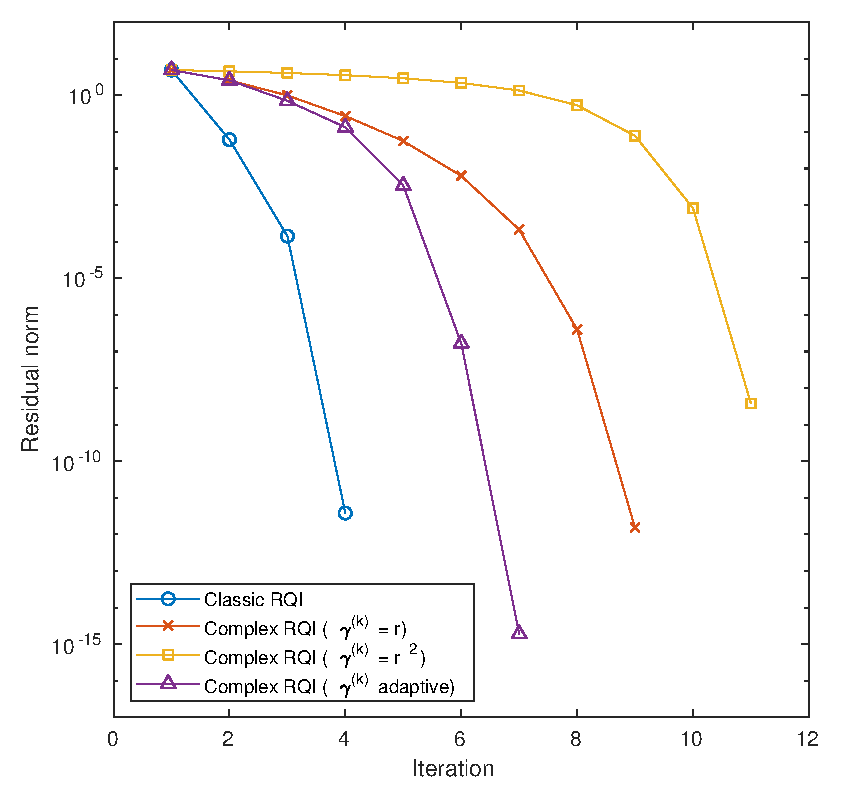
\includegraphics[width=0.7\textwidth]{Figures/crqi_residuals}
  \caption[Residuals for different choices of $\gamma^{(k)}$.]{Plot of
    residuals of Classic RQI, Complex RQI with
    $\gamma^{(k)} = \norm*{\vec{r}^{(k)}}$, Complex RQI with
    $\gamma^{(k)} = \norm*{\vec{r}^{(k)}}^2$ and Complex RQI with the
    imaginary shift chosen adaptively (see text). The last variant
    seems to combine the advantages of the second and third
    alternatives.}%
  \label{fig:residuals}
\end{figure}

We observe that in the initial phase of the iteration, the second
variant (squared residual norm) seems to be slower than the
first. Although it is not clearly observable in the figure, further
investigation of other examples suggested that during the final steps
of the iterations the second version was faster than the
first. Consequently, by combining both approaches and thus changing
the shift adaptively we expect faster convergence. The results are
also plotted in Figure~\ref{fig:residuals} and are in accordance with
the expectation. In this particular case, the shift was changed
according to
\begin{equation*}
  \gamma^{(k)} =
  \begin{cases}
    \norm*{\vec{r}^{(k)}} & \text{ if } \norm*{\vec{r}^{(k)}} \ge 1\,, \\
    \norm*{\vec{r}^{(k)}}^2 & \text{ if } \norm*{\vec{r}^{(k)}} < 1\,.
  \end{cases}
\end{equation*}
In the following, when we speak of CRQI we mean CRQI performed with
this adaptive choice of imaginary shifts.

Running the same experiment but increasing the component of the
initial vector in the direction of the target eigenvector led to a
decrease of the number of additional steps required by CRQI. For
eigenvectors that were very close to the target sometimes both classic
RQI and complex RQI even finished within the same number of
iterations. Still, even in these cases, classic RQI often failed to
converge to the right eigenpair.

In the next examples we will examine how the initial vector and
initial (real) shift affect the results of RQI and CRQI. We have
already discussed the sometimes erratic behaviour of classic RQI. As
we will shortly see, a main problem of RQI is convergence often hardly
depends on the initial vector but rather on the initial shift. This is
why especially for eigenvalue problems with closely spaced eigenvalues
RQI fails to compute the right eigenpair even if the method is started
with a good approximation of the eigenvector. We start with an example
where the algorithm was run many times with a fixed initial vector but
varying initial shifts. To obtain the shifts we computed the spectrum
of the matrix using built-in functions of Matlab and then extracted
100 evenly spaced values form the interval
$[\lambda_{\text{min}} - 10, \lambda_{\text{max}} + 10]$, where
$\lambda_{\text{min}}$ and $\lambda_{\text{max}}$ are the smallest and
largest eigenvalue of $\mat{A}$, respectively. The results are plotted
in Figure~\ref{fig:vary shift}. The initial vector was set to a
weighted combination of the exact eigenvectors as described above.
The component in the target direction was small in the first two
examples (Figure~\ref{fig:varying shift small negative}
and~\ref{fig:varying shift small positive}), big in the third example
(Figure~\ref{fig:varying shift big}) and not larger than the remaining
components in the last example (\ie none of the weights was set to a
larger value than any of the others, Figure~\ref{fig:varying shift
  random}).

\begin{figure}[htpb]
  \centering
  \begin{subfigure}[b]{0.475\textwidth}%
    \centering
    \includegraphics[width=\textwidth]{Figures/crqi_varyingshift__initvec_small_direction_70deg_negative}%
    \caption{{\small Small component in target direction, negative
        eigenvalue}}%
    \label{fig:varying shift small negative}
  \end{subfigure}%
  \hfill
  \begin{subfigure}[b]{0.475\textwidth}%
    \centering
    \includegraphics[width=\textwidth]{Figures/crqi_varyingshift__initvec_small_direction_70deg}%
    \caption{{\small Small component in target direction, positive
        eigenvalue}}%
    \label{fig:varying shift small positive}
  \end{subfigure}
  \vskip\baselineskip
  \begin{subfigure}[t]{0.475\textwidth}%
    \centering
    \includegraphics[width=\textwidth]{Figures/crqi_varyingshift__initvec_suffctl_big}%
    \caption{{\small Sufficiently big component in target direction}}%
    \label{fig:varying shift big}
  \end{subfigure}
  \hfill
  \begin{subfigure}[t]{0.475\textwidth}%
    \centering
    \includegraphics[width=\textwidth]{Figures/crqi_varyingshift__initvec_random}%
    \caption{{\small Random initial vector}}%
    \label{fig:varying shift random}
  \end{subfigure}
  \caption[RQI and CRQI with varying initial shifts]{Plot of initial
    real shift against the computed eigenvalue using classic RQI and
    CRQI. The dotted area encloses the initial shifts that lie in the
    spectrum of $\mat{A}$. In the first two examples the initial
    vector had only a small component in the direction of the target
    eigenvector. }%
  \label{fig:vary shift}
\end{figure}

We observe that RQI seems to depend heavily on the choice of the
initial shift, especially when the shift lies between the upper and
lower bound of the spectrum (indicated by the dotted area in the
plots). This does not change even for initial vectors that are very
close approximations of an eigenvector as we have already seen
earlier, in Section~\ref{sec:rqi:recent}. In contrast, it appears that
CRQI does not depend so much on the shift but rather on the initial
vector. In the first two examples, it seems as if in some cases the
result of CRQI depends on the sign of the target eigenvalue. If the
eigenvalue is negative, shifts below this eigenvalue produced the
correct result whereas shifts above the eigenvalue did not and
analogously for positive eigenvalues. Further investigation revealed
that this has actually nothing to do with the target eigenvalue being
negative or positive but rather its location in the spectrum. If it is
below the centre of the spectrum the behaviour is as in
Figure~\ref{fig:varying shift small negative} and for eigenvalues
above the centre the results are similar to those in
Figure~\ref{fig:varying shift small positive}. This observation could
possibly be used if the initial vector is not that good of an
approximation but some knowledge of the spectrum is available so that
the initial shifts could be chosen accordingly.

We have examined the influence the initial shifts have on the
convergence outcome. The last paramater we can adjust is the initial
vector. In this next example, we study the relationship between the
angle that the initial vector makes with the target eigenvector and
the outcome of the method. To that end, we create an artificial
approximation of the wanted eigenvector as explained above and
succesively increase the contribution in the target direction.  In the
motivational section of this chapter CRQI was introduced as an
improvement of classic RQI in the sense that good approximations of
eigenvectors should lead to convergence to this very eigenvector. The
example confirms the expectations; in particular we will see that
\begin{enumerate}[label=(\alph*)]
\item classic RQI indeed suffers from the problem that good
  approximations of an eigenvector do not necesarrily lead to
  convergence to this right eigenvector and that
\item complex RQI seems to take much more advantage of the information
  in the initial vector.
\end{enumerate}
The results are given in Figure~\ref{fig:angle_test}. We see that
complex RQI seems to converge to the right eigenvector much sooner;
once the angle between the initial vector and the target is
sufficiently small (or the angle between the initial vector and the
sum of the remaining eigenvectors is sufficiently big), CRQI produces
the correct result. Classic RQI, on the other hand, still often
converges to the wrong eigenpair for very small angles. The figure
suggests that ``sufficiently small'' means approximately below
$\pi / 4$.

\begin{figure}[htpb]
  \centering
  \begin{subfigure}[t]{0.45\textwidth}%
    \centering
    \includegraphics[width=\textwidth]{Figures/test_angle_plot}%
    % \caption{{\small Plot of the angle between the target
    % eigenvector
    % and the initial vector and the computed eigenvalue}}%
    \label{fig:angle_test:target}
  \end{subfigure}%
  \hfill
  \begin{subfigure}[t]{0.45\textwidth}%
    \centering
    \includegraphics[width=\textwidth]{Figures/test_angle_plot_rem}%
    % \caption{{\small Plot of the angle between the remaining
    % eigenvectors and the initial vector and the computed
    % eigenvalue}}%
    \label{fig:angle_test:rem}
  \end{subfigure}
  \caption[RQI and CRQI with varying initial vectors]{Plot of the
    computed eigenvalue against the angle between the initial vector
    and the target eigenvector (left) and the remaining eigenvectors
    (right), respectively.}%
  \label{fig:angle_test}
\end{figure}
\todo{Fix caption below right figure}

Test sentences
%%% Local Variables: 
%%% mode: latex
%%% TeX-master: "../../main"
%%% End:
